\chapter{Project Implementation}
% Presentation of project implementation:
% functional diagrams,
% solutions used in the implementation,
% what were the most difficult/interesting parts of the implementation,
% why and how were they implemented (describe any innovative ideas and solutions you included; include code snippets as example if necessary)
In this chapter we will take a closer look at the project implementation.
We will start from with the base infrastructure, continuing with layer 2 up to layer 4 and the BGP messages.
At the end we will explain our T-BGP and hybrid model implementation.\newline
In every section we will describe also the limitations and workarounds that we made to reduce the workload.
Note that thanks to these simplifactions, we have been able to finish the project in six weeks maintaining a very high outcome quality.

\section{Simulator Infrastructure}
To implement our simulator we used plain Java 13.
Specifically, we used Project Reactor for scheduling and PDU delivery, while we used Graphstream for visualization and graph operations.
Moreover, to improve the UI, we decided to use JavaFX to provide more in-dept visualization and some runtime controls like:
\begin{itemize}
    \item Turn off and on a router
    \item Check the router state
    \item View the routes
\end{itemize}
We decided to use a test-driven development (TDD) approach, trying when possible to write the tests as first and then implement the algorithms. \newline
The simulator includes support to export the traffic one or all networks via command line arguments (see \ref{simulatorDoc}). This was used to prove that the protocol implementations were according to standard.\newline
Last but not least, we inserted a TUN device support to open a tunnel into the simulation (Linux only).
In this way, we can directly connect our host computer with a simulated server.

\section{Layer 2}\label{layer2}
Our simulated IEEE 802.3 Ethernet allows an unlimited MTU.
The Preamble, start frame delimiter (SFD), frame check sequence (FCS) and the interframe gap (IFG) are not implemented to reduce the workload and since they are not required for the PCAP export.
Given that the project is in a simulation environment, all these components were not necessary for the required functionality.\newline
We also implemented data structures and algorithms to support operations which are normally solved by other protocols:
\begin{itemize}
    \item Support to resolve IP addresses (replacing the ARP protocol)
    \item Support to enumerate devices on a network (Neighbor Discovery Protocol replacement)
\end{itemize}


\section{Layer 3}\label{layer3}
For what concerns the Network Layer we first created the IPv6 header following the RFC 2460 \cite{rfc2460}.\newline
To be sure that the implementation was correct we created several unit tests to check that the IP packet was parsed correctly.
Moreover, we tried to exchange messages using Wireshark and we noticed that everything was correct.\newline
Then, to simplify the implementation we get rid of the traffic class and the flow label, which are both set to 0.
Note that we do not need them for the BGP implementation itself.
\par About the routing, we initiate the simulation using a YAML document and from that, we generate the local static routes.\newline
Once the system is running, the routing tables are updated by the routers through the BGP messages.
The path to delivering a packet is based on the prefix match, where we consider the length of the prefix as discussed in the lectures.\newline
In case the prefix is equal, we calculate a second parameter.
It can be the route metric (if set), or the result of our formula, which takes the AS\_PATH length multiplied by 100 and divides the result by the neighbour trust.
Therefore, the more we trust the next-hop, the smaller the calculated parameter will be and the higher the probability that route will be chosen is.

\section{Layer 4}\label{layer4}
About the Transport Layer, we decided to implement the TCP header following the RFC 793 \cite{rfc793}.
Also, in this case, we used some default values like the Urgent Pointer, the Options and the relative Padding since we do not need them for this application.\newline
One fundamental limitation is that our TCP implementation is message-based since it was not the main goal of the project and it was a lot easier.
Therefore, there is not data buffer and it can be considered like a UDP protocol but with the TCP header.
Moreover, we did not implement any error handling or retransmission technique.\newline
Nevertheless, we implemented the 3WHS to establish the connection and the FIN based messages to close it.

\section{BGP Messages}\label{BGPMex}
The BGP implementation follows quite specifically the RFC 4271 specification, which define four different kind of messages.
In the next paragraphs there will be a brief recap of required fields for KEEPALIVE, OPEN and NOTIFICATION messages. It's noteworthy to spend more time explaining the implementation of the UPDATE message, which is not trivial as the others due to the taken design decision of using IPv6 rather then the default IPv4.

Each message need to integrate an header, composed by three simple fields:
\begin{itemize}
    \item \texttt{Marker} (16 bytes): each bit is set to 1;
    \item \texttt{Length} (2 bytes): number of bytes of the message, this header included;
    \item \texttt{Type} (1 byte): specify which of the 4 messages is following the header.
\end{itemize}

\subsection{OPEN Message}
The OPEN message is the one used to enstablish a connection need to be sent by both parties of the connection.
The message is composed by the following fields:
\begin{itemize}
    \item \texttt{Version} (1 byte): the protocol version number, in this project it is 4;
    \item \texttt{My Autonomous System} (2 bytes): identifier number of the sender;
    \item \texttt{Hold Time} (2 bytes): proposal of Hold Time interval;
    \item \texttt{BGP Identifier} (4 bytes);
    \item \texttt{Optional Parameters Length} (1 byte);
    \item \texttt{Optional Parameters} (variable length).
\end{itemize}


\subsection{KEEPALIVE Message}
This message is used when a well-formatted OPEN message is received and need to be sent regularly to avoid the expiration of the Hold Timer. The suggested interval is a third of the Hold Timer. In this project, the Hold Timer expires after 90 seconds of no received KEEPALIVE, which is sent every 30 seconds. No extra fields are included, therefore the 19 byte message header is the sole content of this message.


\subsection{NOTIFICATION Message}
When an error is detected, a NOTIFICATION message is sent. Three are the needed fields for this message:
\begin{itemize}
    \item \texttt{Error code} (1 byte);
    \item \texttt{Error subcode} (1 byte);
    \item \texttt{Data} (variable length).
\end{itemize}
Immediatly after the message, the connection is closed.

\subsection{UPDATE Message}
As anticipated before, this message required more effort to be implemented because of the requirement to be complient with IPv6.
Therefore, the message is still based on the RFC 4271 \cite{rfc4271}, but apply necessarly take into account some extra path attributes described in the RFC 1812 \cite{rfc1812} specification.
Specified fields from RFC 4271 are:
\begin{itemize}
    \item \texttt{Withdrawn Routes Length} (2 bytes);
    \item \texttt{Withdrawn Routes} (variable);
    \item \texttt{Total Path Attribute Length} (2 bytes);
    \item \texttt{Path Attributes} (variable);
    \item \texttt{Network Layer Reachability Information} (variable).
\end{itemize}
In the standard implementation, \texttt{Withdrawn routes} and \texttt{network layer reachability information} need to be specified as IPv4 addresses in the relative fields of the message itself. Instead, the \texttt{Path attributes} field need to be fullfilled with at least 3 sub-fields which are \texttt{origin}, \texttt{next hop} and \texttt{as path}.
RFC 1812 permit to include two additional sub-fields to \texttt{path attributes}, indicating \texttt{withdrawn routes} and \texttt{network layer reachability information} in a IPv6 format.
This means that:
\begin{itemize}
    \item The \texttt{withdrawn routes length} can take value 0;
    \item Consequently, the \texttt{withdrawn routes} can be left empty;
    \item In the same way, also \texttt{network layer reachability information} won't be present anymore.
\end{itemize}
In turn, two additional subfields are specified:
\begin{itemize}
    \item \texttt{MP\_REACH\_NLRI}, where network layer reachability information is specified together with the \texttt{next hop}.
    \item \texttt{MP\_UNREACH\_NLRI}, containing the withdrawn routes.
\end{itemize}

\section{Finite State Machine}\label{fsm}
Each router holds a \texttt{Finite State Machine} for each peer connection it has. The FSM contains all the parameters needed to perform the connection, send messages and manage the context. It describes what actions should be taken by the BGP routing engine and when.\\
It has been implemented using the \textit{Squirrel Foundation}\footnote{\url{https://github.com/hekailiang/squirrel}} Java library, an open source project which provides a lightweight and easy-to-use state machine implementation.\\
Since only one peer needs to open the connection, we implemented a naive collision avoidance algorithm that selects, as node initiator of a connection, the one that has the lower IP address. This approach is not exactly correct, but it works well for our purposes.\\
As stated in RFC 4271 \cite{rfc4271}, the finite state machine can be in six different states, each one performing specific actions. The transition between one state to another is fired by events (all the transitions are implemented, but not all the error events are fired to simplify the implementation), and each of them holds callback functions.\\
We also implemented the three mandatory timers (\texttt{ConnectRetryTimer}, \texttt{HoldTimer} and \texttt{KeepaliveTimer}), plus the \texttt{DelayOpenTimer}, by following the specification of RFC 4271.

\section{Graphical User Interface}
The GUI is essential to give the user the possibility to interact with the simulation and turn on/off nodes, inspect the routing tables and the state of the finite state machines.\\
As you can see from Fig. \ref{fig:gui}, on the left side of the window it is shown the graph of the network infrastructure which can be dragged and arranged as wanted. By clicking on a node, on the right hand side we can see the information about it, such as the BGP peers connection status and the routing table. Pressing the "Shutdown" button it is possible to turn off the node and the information in the tables will be refreshed accordingly. 
On the bottom side, there is a console that logs any error occurring.
\begin{figure}[h]
    \centering
    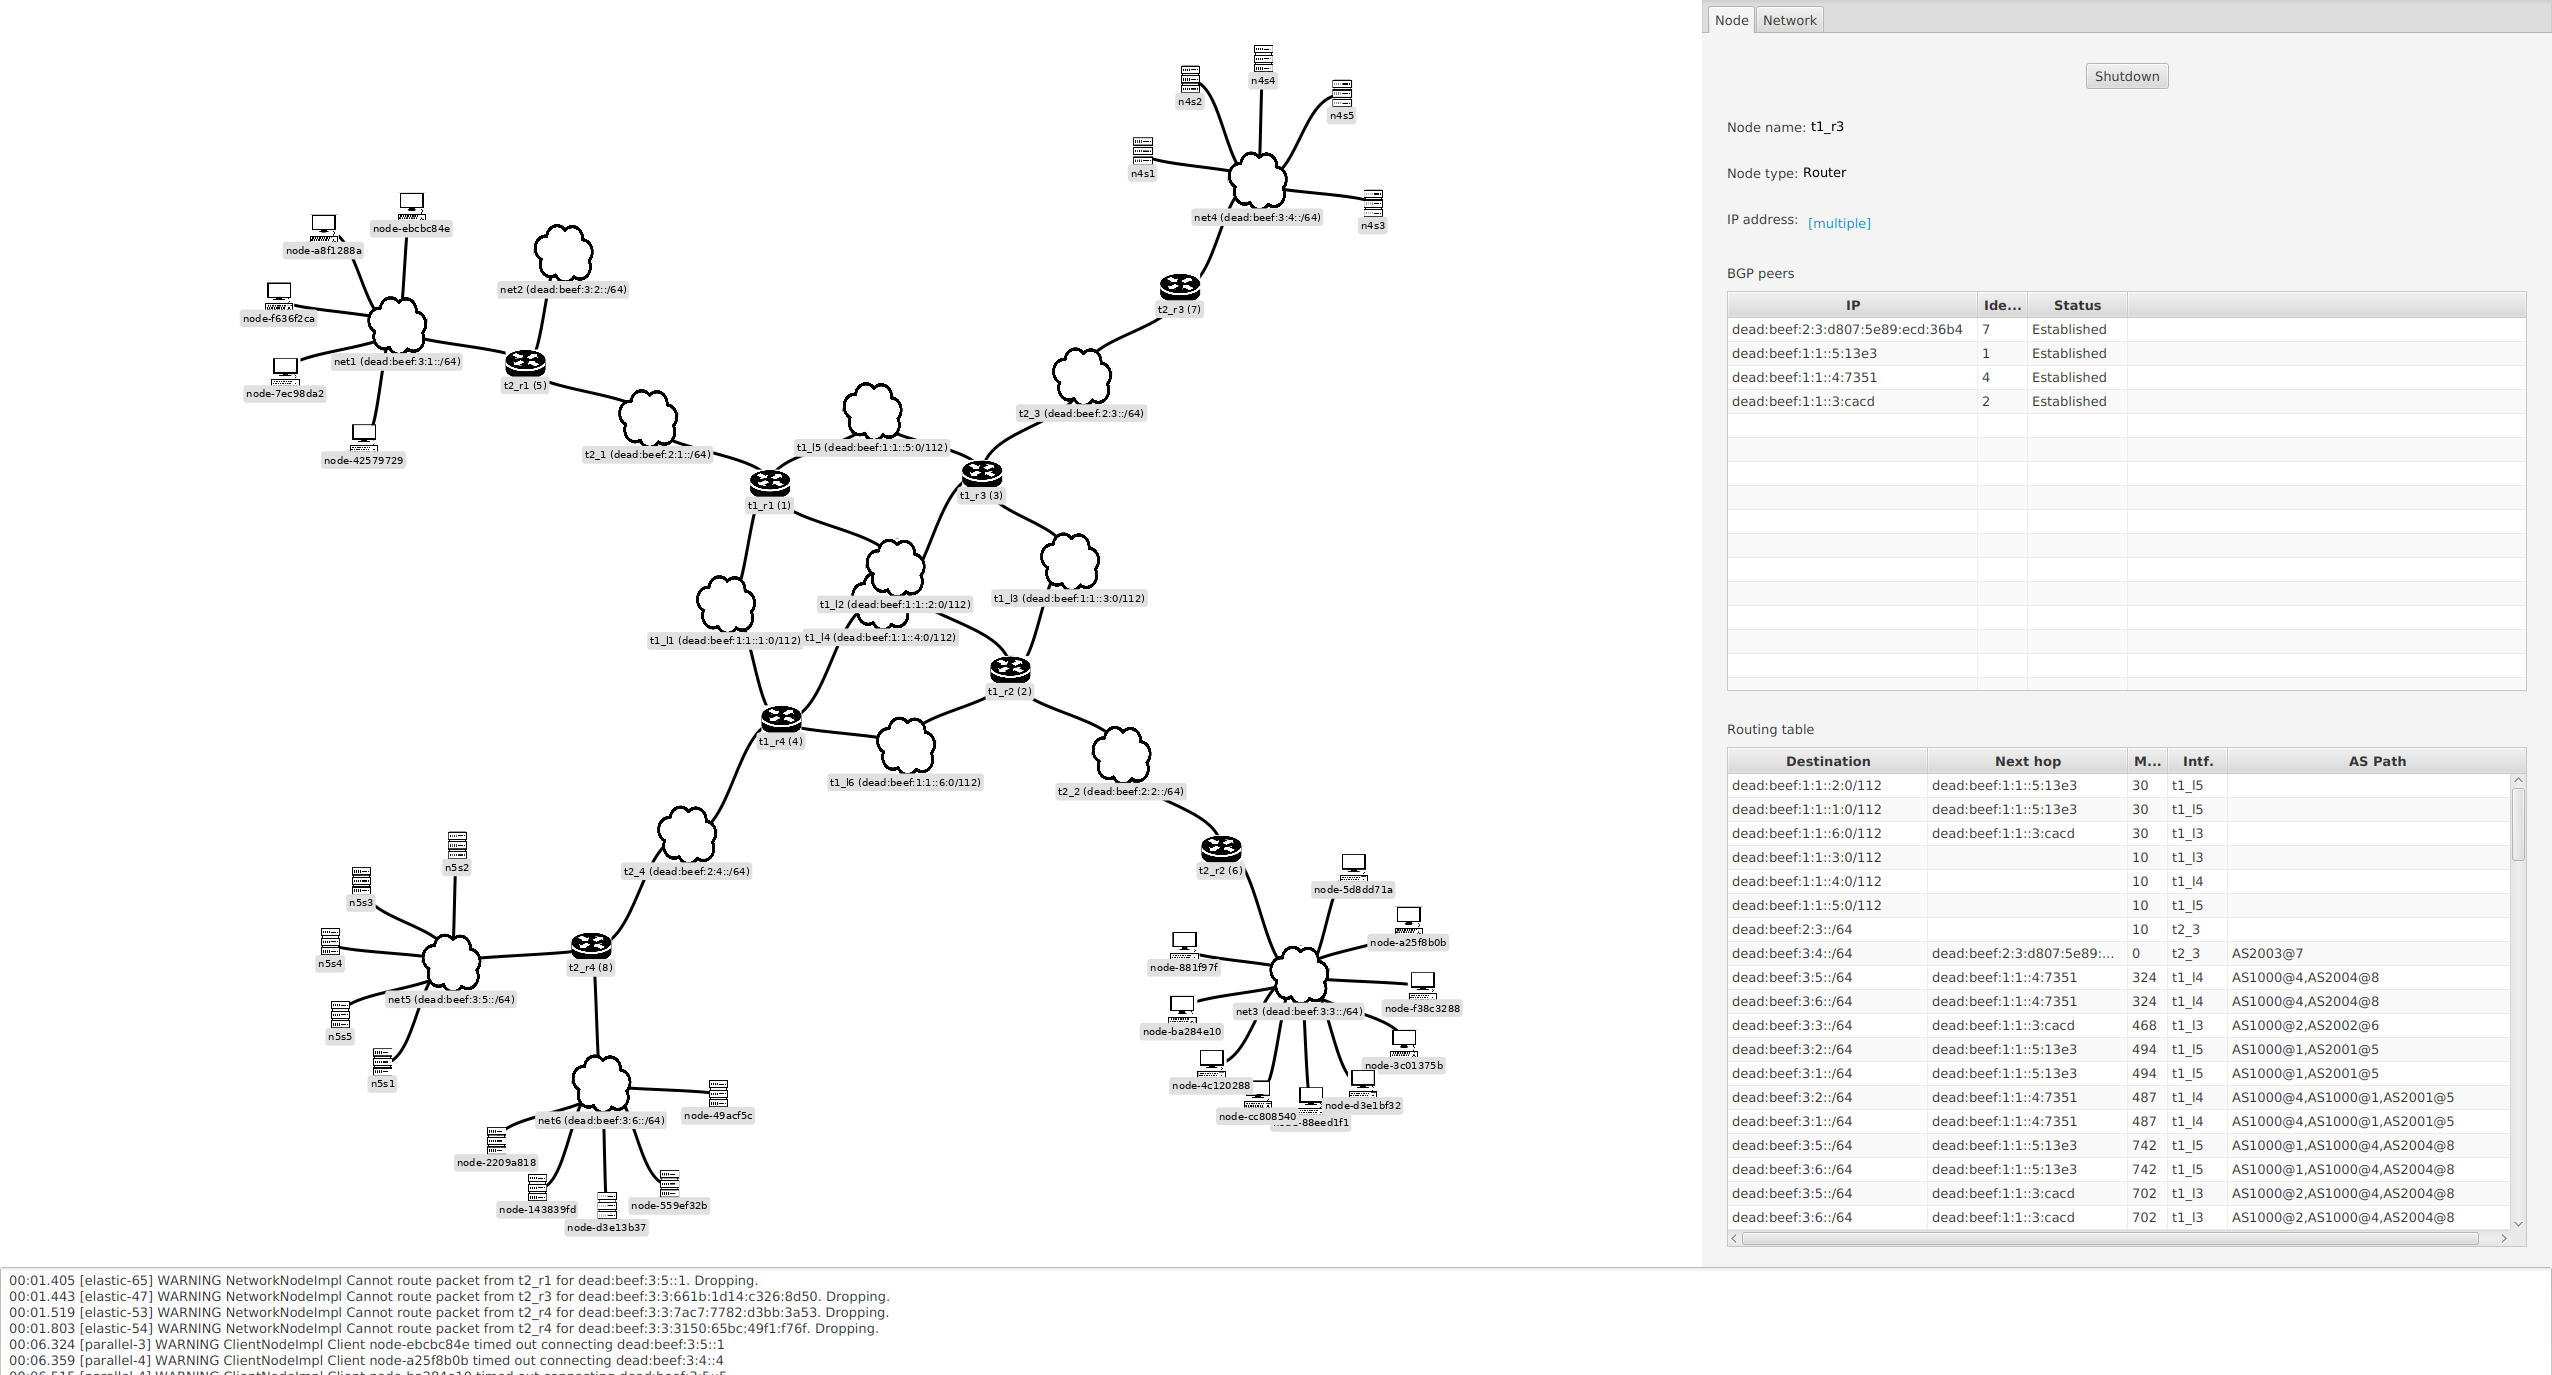
\includegraphics[width=1.0\textwidth]{gui1.png}
    \caption{Graphical User Interface}
    \label{fig:gui}
\end{figure}


\section{T-BGP And Hybrid Model Implementation}\label{BGPTrust}
In the development process of the BGP protocol, trust in between different routers has been taken into account. The followed approach is a conjunction of \textit{Direct} and \textit{Voted Trust}. In the first one, the main focus has been concentrated in the well-known trust model for inter-domain in routing\cite{he2006novel} discussed by \textit{Liwen He}, where Direct Trust is calculated combining \textit{Observed} and \textit{Inherent Trust}.\\
In our implementation, the Inherent Trust is randomly initialized at the startup phase, while the Observed one has a fixed 0.5 default value. Thus, the Observed Trust value vary during the execution of the simulation depending on the neighbor's behaviors: when a KEEPALIVE message is received, the value is increased by 5\%, while in case of connection closure a 10\% reduction is applied.

On the other hand, the realized implementation of the \textit{Voted Trust} follows the baseline provided by the Hybrid Trust Model\cite{rantala2011hybrid}. To realize such system, a specific TCP connection has been established in order to communicate together with the second level neighbors. To achieve so, each party need also to keep an updated list of the second level neighborhood to establish the \textit{Trust Agent} connection, as well as all the updated votes collected from the connections. The peer context has been chosen as the best place where to store such values.

All this values are combined together in order to create a more reliable and precise idea over the neighbor. The calculation follows the formula:
$$ \left\{[(Inherent Trust + Observed Trust) / 2 ] + Voted Trust \right\} / 2 $$
It's trivial to understand that the result is the mean between voted and direct trust, the latter composed in turn of the average between inherent and observed trust.
